\documentclass[11pt,a4paper]{article}
\usepackage[margin=22mm,headheight=14pt]{geometry}
\usepackage{fontspec}
\setmainfont{Latin Modern Roman}
\setsansfont{Latin Modern Sans}
\setmonofont{Latin Modern Mono}
\usepackage{amsmath,amssymb,amsthm}
\usepackage{graphicx,booktabs,array,xcolor,fancyhdr,enumitem}
\usepackage[font=small,labelfont=bf]{caption}
\usepackage[colorlinks=true,urlcolor=teal,linkcolor=teal,citecolor=teal]{hyperref}
\hypersetup{pdftitle={The Adler Fractal: A Recursive Radial Drawing and Its Polygon-IFS Limits},pdfauthor={Marcus Adler},pdfsubject={Technical report version 1.0.0 prepared 30 September 2026}}
\definecolor{ink}{HTML}{243D55}
\definecolor{teal}{HTML}{23858B}
\pagestyle{fancy}
\fancyhf{}
\fancyhead[L]{\small\sffamily\color{ink} ADLER FRACTAL}
\fancyhead[R]{\small\sffamily Technical report \textbar\ 30 September 2026}
\fancyfoot[C]{\small\sffamily\thepage}
\renewcommand{\headrulewidth}{0.3pt}
\setlength{\parindent}{0pt}
\setlength{\parskip}{5.5pt}
\setlist{nosep,leftmargin=*}
\newtheorem{proposition}{Proposition}
\newcommand{\C}{\mathbb C}
\newcommand{\R}{\mathbb R}
\newcommand{\Z}{\mathbb Z}
\newcommand{\dimH}{\dim_{\mathrm H}}
\newcommand{\sectiontitle}[1]{\section*{\sffamily\color{ink}#1}}
\graphicspath{{../figures/}}

\begin{document}

% Page 1
{\sffamily\color{teal}\small TECHNICAL REPORT \quad SPECIFICATION AND SOFTWARE v1.0.0}
\vspace{5mm}

{\sffamily\color{ink}\LARGE\bfseries The Adler Fractal\par}
\vspace{2mm}
{\sffamily\large A Recursive Radial Drawing and Its Polygon-IFS Limits\par}
\vspace{4mm}
{\large Marcus Adler\par}
{\small Version 1.0.0, prepared 30 September 2026. Not independently peer reviewed.\par}
{\small Zenodo DOI: \texttt{10.5281/zenodo.23057945} (reserved before deposition).\par}

\sectiontitle{Abstract}
We document the radial recursive drawing supplied by Marcus Adler under the
proposed name \emph{Adler Fractal}. Every node draws equally spaced spokes in
the same absolute directions; subsequent generations begin at their endpoints.
The original uses 72 directions, two generations and unchanged segment length.
We separate the accumulated trace, the endpoint sets and their closures. We
derive command counts, endpoint multiplicities and sharp radius bounds. For
the equal-length original, the union of all endpoint generations is dense in
the plane. Contractive variants produce established regular polygon iterated
function systems; their trace closures are established inhomogeneous
self-similar sets. A headless Python implementation, original-source comparison,
proofs and reproducible figures accompany this report. No claim of a new
mathematical fractal family or historical priority is made.

\begin{center}
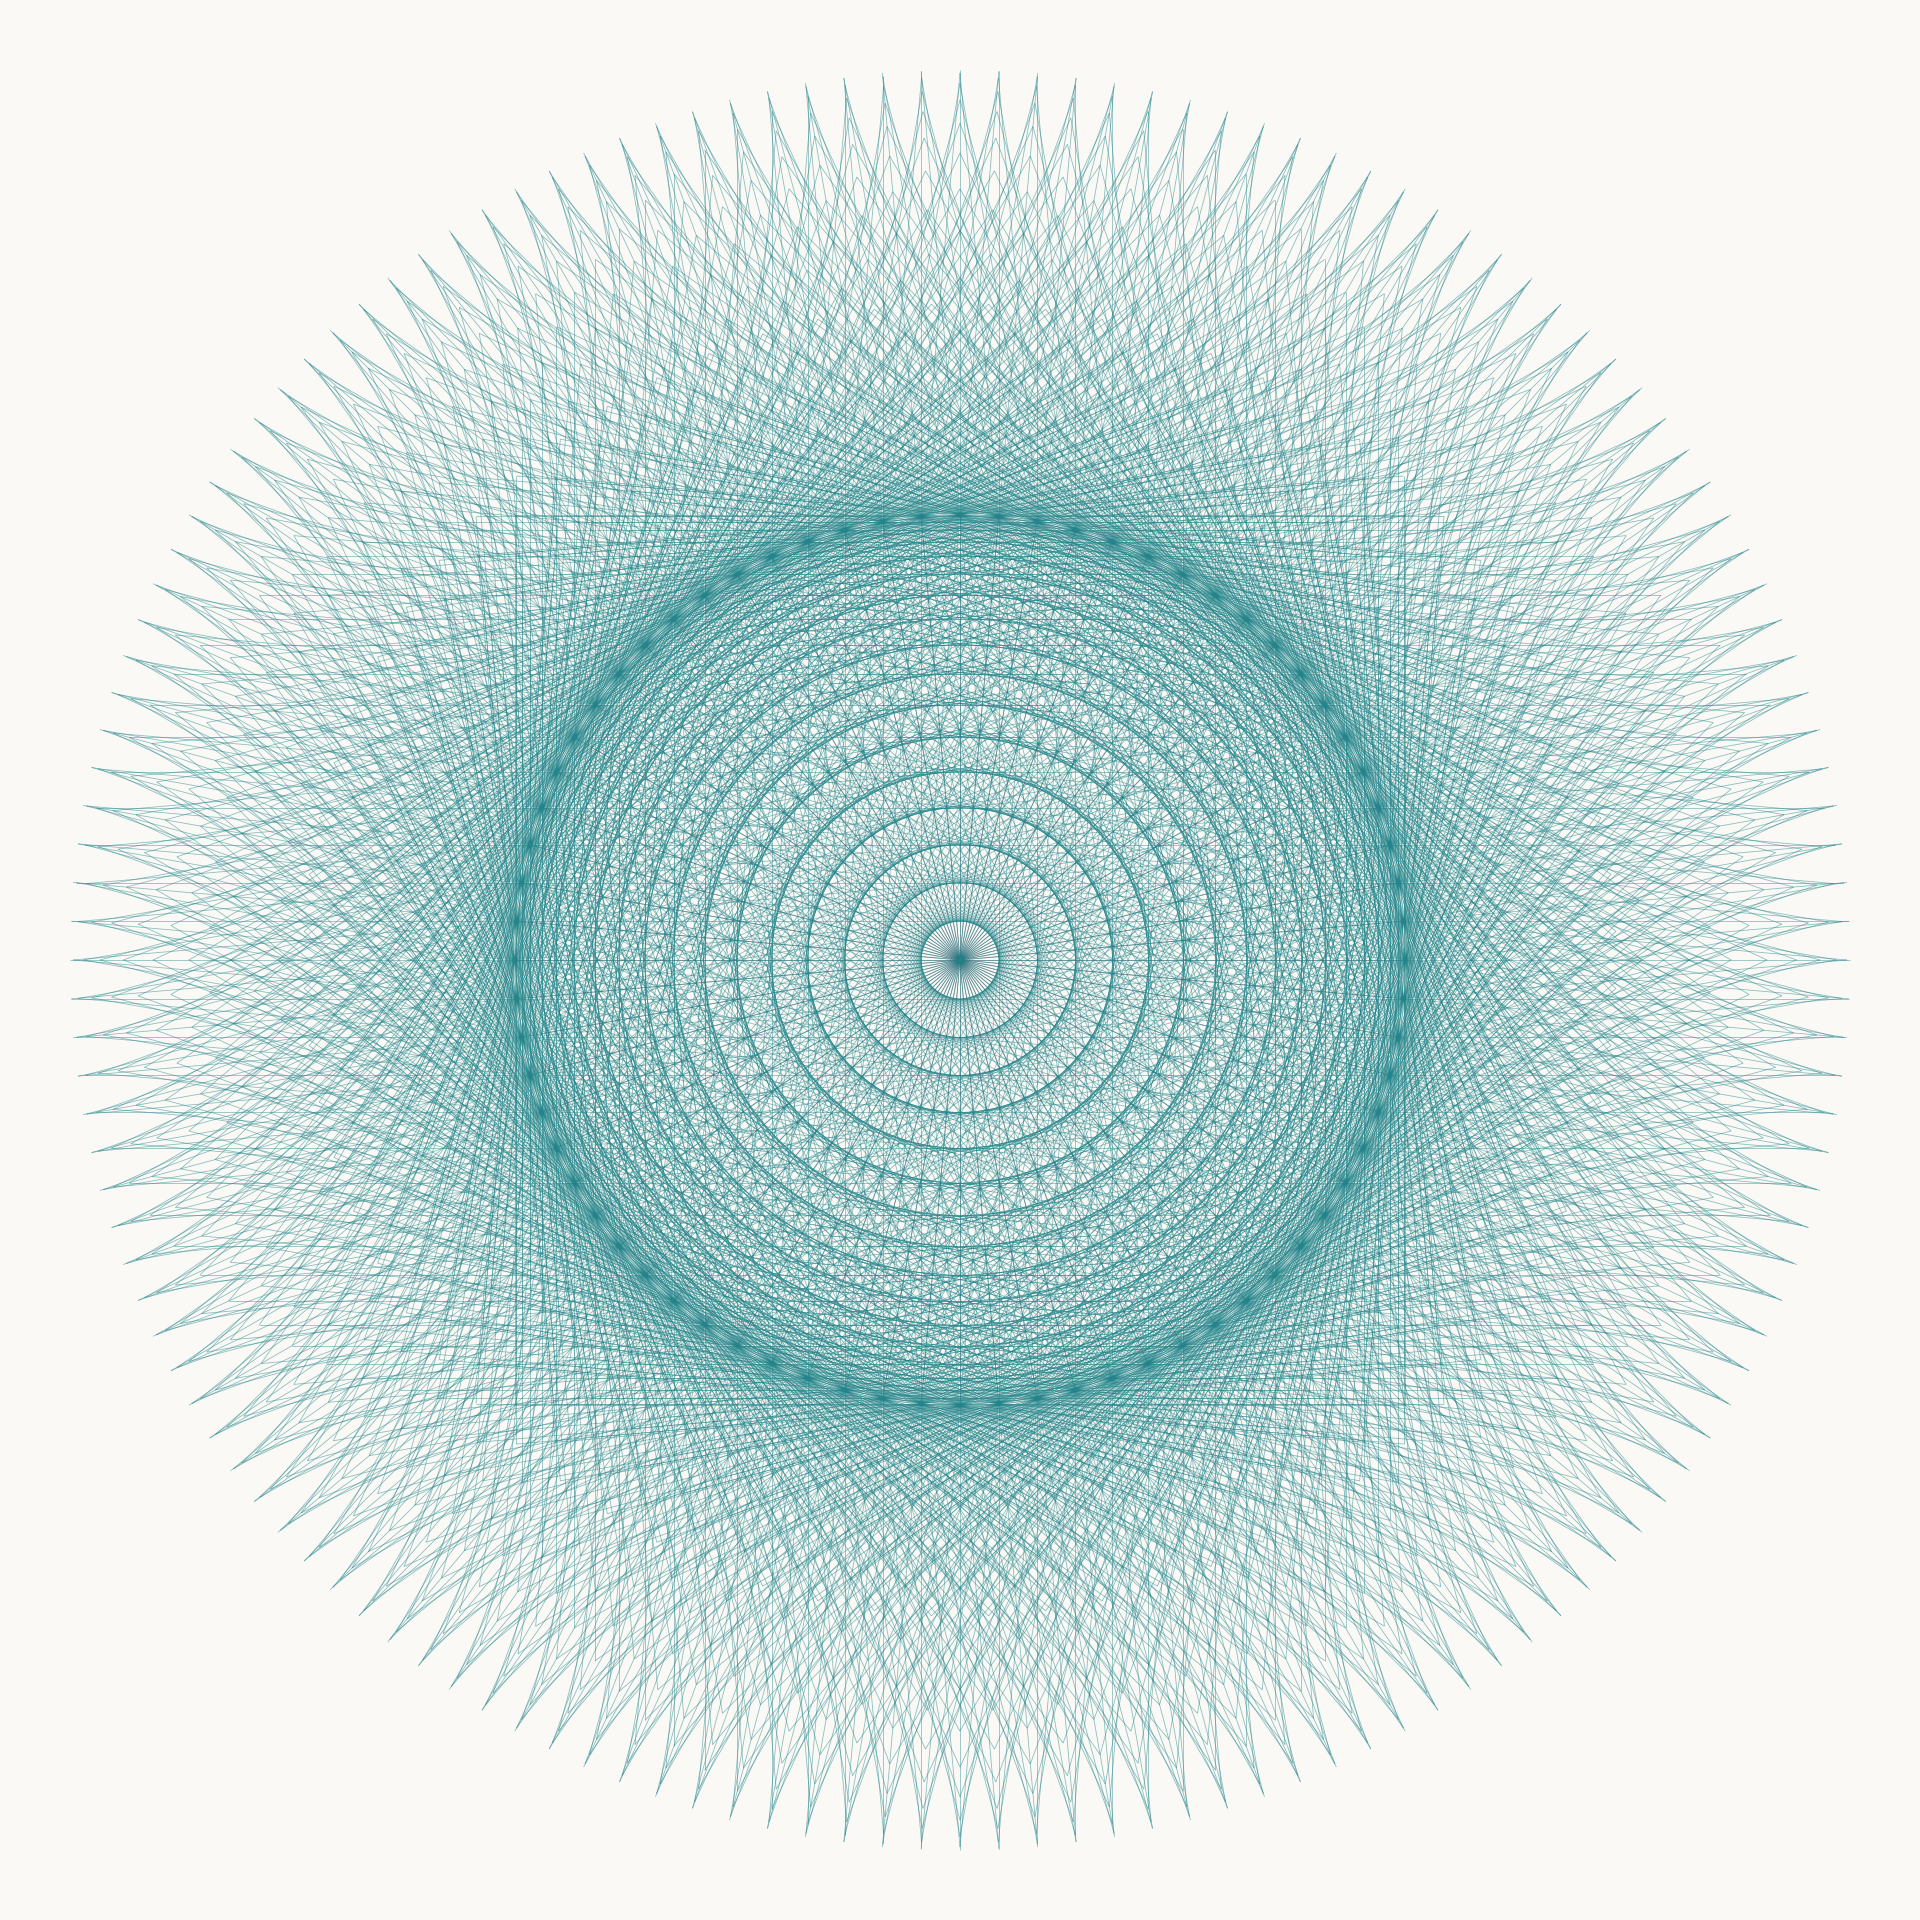
\includegraphics[width=98mm]{adler_original.png}
\captionof{figure}{Original geometry: $m=72$, $n=2$, $L=200$, $r=1$.
The 5,256 drawing commands create a dense radial rosette. Color and stroke
width are rendering choices, not part of the geometric definition.}
\end{center}

{\small\textbf{Provenance.} The unchanged supplied file is archived as
\texttt{original/eagle\_fractal.py}. Formalization, analysis, draft text and
reference software were prepared with assistance from OpenAI ChatGPT.
Independent mathematical review has not been performed.}

\newpage
% Page 2
\sectiontitle{1. Definition and relation to the supplied program}
Identify the Euclidean plane with $\C$. Fix an integer $m\ge3$, a depth
$n\ge0$, an initial length $L>0$, a scale $0<r\le1$, an orientation
$\theta\in\R$ and an origin $z_0\in\C$. Define
\[
u_j=e^{i(\theta+2\pi j/m)},\qquad j=0,\ldots,m-1.
\]
The same global directions are used at every node. No direction is rotated
relative to the incoming segment. For a word $w=(j_1,\ldots,j_k)$, put
\begin{equation}
p_w=z_0+L\sum_{t=1}^k r^{t-1}u_{j_t},\qquad p_\emptyset=z_0.
\end{equation}
Let $w^-$ be the word with its last symbol removed. Define the generation-$k$
endpoint set and the accumulated trace by
\begin{align}
E_k&=\{p_w:|w|=k\},\\
A_n&=\bigcup_{k=1}^n\ \bigcup_{|w|=k}[p_{w^-},p_w],\qquad A_0=\emptyset.
\end{align}
Here $[a,b]$ denotes a closed straight segment. An endpoint can have several
addresses. Coincident drawing commands count separately in a program, but
the geometric union contains each point only once.

For $z_0=0$, write
\[
B=\bigcup_{j=0}^{m-1}[0,Lu_j],\qquad f_j(x)=Lu_j+rx.
\]
The finite trace satisfies
\begin{equation}
A_n=B\cup\bigcup_{j=0}^{m-1} f_j(A_{n-1}).
\end{equation}
Other origins translate all sets by $z_0$. Subsequent sections use origin zero.

\subsection*{Original parameters and traversal}
The supplied main call has
\[
(m,n,L,r,\theta,z_0)=(72,2,200,1,0,0),\quad \alpha=360^\circ/m=5^\circ.
\]
At a node, all $m$ spokes are drawn first in increasing angle order.
The children are then visited recursively in the same order. Repositioning
between segments happens with the pen raised. The reference generator
preserves this ordering, including retraced segments.

The original accepts integer steps in \texttt{range(0, 360, ang)}. If the
step does not divide 360, the cyclic gap at the end differs from the other
gaps. Such nonregular direction sets are outside this specification; the
angle-import adapter rejects them explicitly. The default function argument
in the supplied file is 20 degrees, while its actual main call uses 5 degrees.

The drawing function receives \texttt{\_turtle} but accesses a global
\texttt{turt}. The new adapter uses the provided object. The original file
is preserved unchanged; the correction changes the dependency, not the
intended geometry of its supplied main call.

\newpage
% Page 3
\sectiontitle{2. Finite counts, geometry and multiplicity}
\begin{proposition}
The number of drawing commands and their total length, with multiplicity, are
\[
N_n=\sum_{k=1}^n m^k=\frac{m(m^n-1)}{m-1},\qquad
T_n=Lm\sum_{k=0}^{n-1}(mr)^k.
\]
The sharp outer radius is $R_n=nL$ for $r=1$ and
$R_n=L(1-r^n)/(1-r)$ for $0<r<1$.
\end{proposition}
\begin{proof}
Generation $k$ has $m^k$ addresses and length $Lr^{k-1}$ per command.
Summing gives the first two formulas. The triangle inequality bounds every
endpoint by $R_n$; a word repeating a single direction attains it. The ball
of that radius also contains all segments, by convexity.
\end{proof}

\begin{center}
\begin{tabular}{r r r}
\toprule
Depth $n$ & Commands, $m=72$ & Outer radius, $L=200$, $r=1$\\
\midrule
1 & 72 & 200\\
2 & 5,256 & 400\\
3 & 378,504 & 600\\
4 & 27,252,360 & 800\\
\bottomrule
\end{tabular}
\end{center}
In particular, $T_2=1,051,200$ length units for the original. This is not
the length of the trace after removing overdraw.

\subsection*{Symmetry and finite dimension}
Rotation through $2\pi/m$ permutes the direction indices. Reflection in an
axis through a direction does likewise. Thus $A_n$ and $E_n$ are invariant
under the corresponding dihedral group. For $n\ge1$, $A_n$ is connected:
each new star attaches at an endpoint of an earlier segment. It is a finite
union of nondegenerate segments, so $\dimH A_n=1$.

\subsection*{Why the second generation looks circular}
For $r=1$ and $n=2$,
\[
|p_{(a,b)}|=L|u_a+u_b|
=2L\left|\cos\frac{\pi(a-b)}m\right|.
\]
These discrete radii explain the rings in the endpoint pattern. They do not
assert that entire circles are present in the trace.

For even $m$, the second endpoint set has exactly $m^2/2+1$ distinct points.
Indeed, a nonzero midpoint of a chord of a fixed circle uniquely determines
its unordered endpoints. There are $m(m+1)/2$ unordered pairs allowing
repetition; all $m/2$ antipodal pairs collapse to zero, and all other pairs
remain distinct. Hence the count is $m(m+1)/2-m/2+1$. For $m=72$, 5,184
endpoint addresses therefore represent only 2,593 points. The origin has
72 ordered addresses.

\newpage
% Page 4
\sectiontitle{3. The infinite equal-length original is dense in the plane}
This section concerns the union over \emph{all} depths, not the finite
picture on page 1. Keep $m=72$, $r=1$ and $\theta=0$.

\begin{proposition}
The union of all endpoint generations is dense in $\R^2$. Consequently,
\[
\overline{\bigcup_{n\ge1}A_n}=\R^2.
\]
The unclosed endpoint union has Hausdorff dimension zero, the unclosed
trace union has dimension one, and the closed trace union has dimension two.
\end{proposition}
\begin{proof}
Every direction has its opposite in the 72-direction set. The union
$G=\bigcup_{k\ge0}E_k$ is therefore the additive group generated by the
vectors $Lu_j$: every integer linear combination is a finite sum using
positive or opposite directions.

In units of $L$, directions at 0, 30, 60 and 90 degrees belong to this set,
and
\begin{align*}
2u_{30^\circ}-u_{90^\circ}&=(\sqrt3,0),\\
2u_{60^\circ}-u_{0^\circ}&=(0,\sqrt3).
\end{align*}
The unit axis vectors also occur. Thus
\[
L(\Z+\sqrt3\Z)\times L(\Z+\sqrt3\Z)\subset G.
\]
The subgroup $\Z+\sqrt3\Z$ is dense in $\R$. To see this directly,
the pigeonhole principle applied to the fractional parts of
$0,\sqrt3,\ldots,N\sqrt3$ gives a nonzero group element of magnitude
less than $1/N$. It is nonzero because $\sqrt3$ is irrational. Changing
its sign makes it positive; its integer multiples approximate any real
number within that magnitude. The product of the two dense subgroups is
dense in the plane.

Every endpoint belongs to a trace, so the trace closure is the plane as
well. The endpoint union is countable. The trace union is a countable
union of segments and contains a nondegenerate segment. Countable
stability of Hausdorff dimension gives dimensions zero and one,
respectively. The plane has dimension two.
\end{proof}

\begin{center}
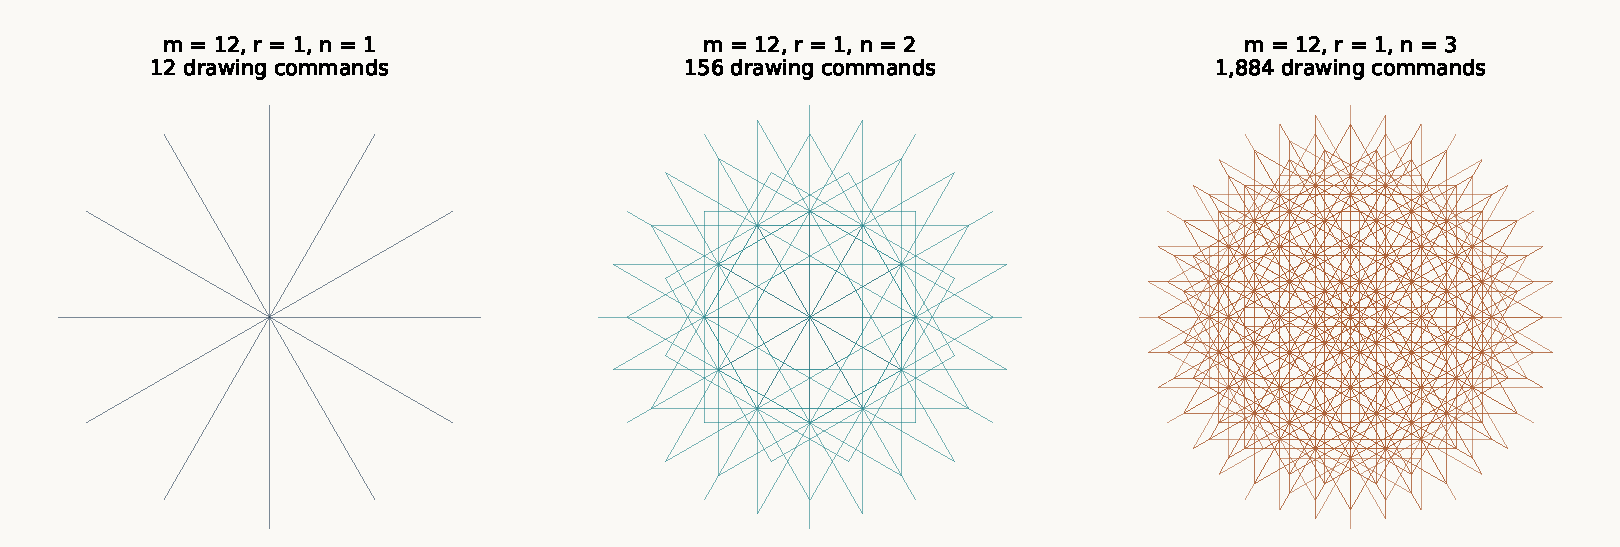
\includegraphics[width=\linewidth]{equal_length_stages.pdf}
\captionof{figure}{Three finite stages with 12 directions, a subset of the
72-direction set containing the same axis and 30-degree directions used
in the proof. Each panel is scaled to its own radius. Finite images do
not by themselves prove density.}
\end{center}

The outer radius grows as $nL$. There is no bounded compact attractor in
this equal-length case, and compact-set Hausdorff convergence to a bounded
limit is not available. Density is a property of the union's closure;
it does not make the unclosed countable endpoint union two-dimensional.

\newpage
% Page 5
\sectiontitle{4. Contractive endpoints: an established polygon IFS}
For $0<r<1$, define the infinite endpoint set
\begin{equation}
K=\left\{L\sum_{t=1}^{\infty}r^{t-1}u_{j_t}:
j_t\in\{0,\ldots,m-1\}\right\}.
\end{equation}
The series converges uniformly over addresses. Its image is compact and
satisfies $K=\bigcup_j f_j(K)$ for $f_j(x)=Lu_j+rx$; it is the unique
nonempty compact attractor of these contractions, as in the standard
IFS theory of Hutchinson \cite{hutchinson}.

Set $v_j=Lu_j/(1-r)$. Then
\begin{equation}
f_j(x)=rx+(1-r)v_j=v_j+r(x-v_j).
\end{equation}
These are precisely contractions about vertices of a regular polygon.
Polygon-vertex systems, polygonal seeds and star-shaped seeds already
appear in the literature, for example Tzanov \cite{tzanov}. This change
of coordinates and notation does not create a new endpoint-IFS family.

The convex hull of $K$ is the regular polygon with vertices $v_j$.
Every series is $L/(1-r)$ times a convex combination of the $u_j$;
each vertex occurs as a constant address. Truncating and extending
addresses yields the explicit approximation bound
\begin{equation}
d_H(E_n,K)\le\frac{Lr^n}{1-r}.
\end{equation}

\subsection*{A sufficient separation certificate}
Each $f_j(K)$ lies in the closed disk centered at $Lu_j$ with radius
$rL/(1-r)$. Neighboring centers have distance $2L\sin(\pi/m)$.
Consequently, these disks, and hence the first-level pieces, are disjoint if
\begin{equation}
r<q_m:=\frac{\sin(\pi/m)}{1+\sin(\pi/m)}.
\end{equation}
This sufficient criterion is not a necessary threshold for separation.
Under it, an open disk of radius $L/(1-r)$ is mapped into itself with
disjoint images, giving the open set condition. The standard similarity
dimension theorem \cite{hutchinson} then gives
\begin{equation}
\dimH K=s:=\frac{\log m}{\log(1/r)}.
\end{equation}
Without a verified separation condition, only the general bound
$\dimH K\le\min\{2,s\}$ is asserted here. In particular, $m=72$, $r=1/2$
gives $s\approx6.169925$, which cannot be a planar Hausdorff dimension.

For $m=72$, $q_m\approx0.0417962601$. The choice $r=0.03$ therefore
has the certified dimension $\dimH K\approx1.219619423$. No
pixel-based estimate is used in this conclusion.

\newpage
% Page 6
\sectiontitle{5. The accumulated trace has a different limit}
Let $O=\bigcup_{n\ge1}A_n$ and $S=\overline O$ for $0<r<1$.
The persistent initial star prevents identification of the accumulated
trace with the endpoint attractor alone.

\begin{proposition}
The closed trace is
\[
S=O\cup K=B\cup\bigcup_j f_j(S),\qquad
\dimH S=\max\{1,\dimH K\}.
\]
For $n\ge1$, $d_H(A_n,S)\le Lr^n/(1-r)$.
\end{proposition}
\begin{proof}
Every infinite address is approximated by its endpoints, so $K\subset S$.
For a convergent sequence of trace points, bounded generations stay in
a finite closed union of segments. For unbounded generations, the
distance from a point on a generation-$k$ segment to an infinite
extension of that address is at most $Lr^{k-1}/(1-r)$, which tends to
zero. Thus every remaining limit point lies in $K$, proving $S=O\cup K$.
Taking closures in the finite recursion gives the displayed set equation.
The countable segment union has dimension one. Countable stability gives
the dimension formula. Points in later generations and in $K$ lie
within $Lr^n/(1-r)$ of their depth-$n$ prefixes in $A_n$.
\end{proof}

This is a specialization of the established inhomogeneous self-similar
construction with condensation set $B$, including its usual
homogeneous-plus-orbital decomposition and Hausdorff-dimension rule
\cite{fraser}. These identities are not presented as new general theorems.

\begin{center}
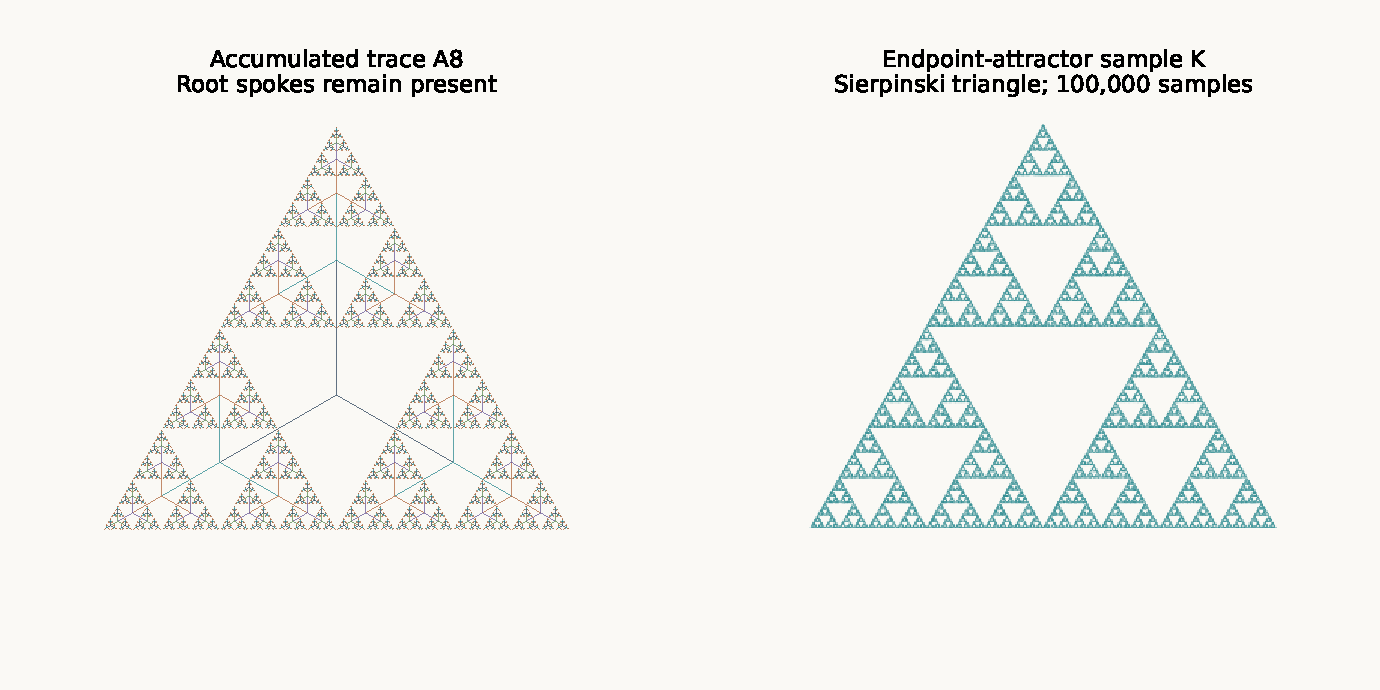
\includegraphics[width=\linewidth]{trace_vs_endpoints.pdf}
\captionof{figure}{$m=3$, $r=1/2$, $L=1$. Left: the trace through
eight generations, including persistent spokes. Right: a finite chaos-game
sample of the classical Sierpinski endpoint attractor. The two sets share
the same closed-limit Hausdorff dimension, but are different sets.}
\end{center}

An endpoint dust can have dimension below one, while its accumulated
trace closure still has dimension one. For example $m=8$, $r=0.1$
gives $\dimH K=\log 8/\log 10\approx0.903090$ and $\dimH S=1$.
Connectedness of the trace and disconnectedness of many endpoint
attractors are compatible with these dimension statements.

\newpage
% Page 7
\sectiontitle{6. Representative endpoint variants}
\begin{center}
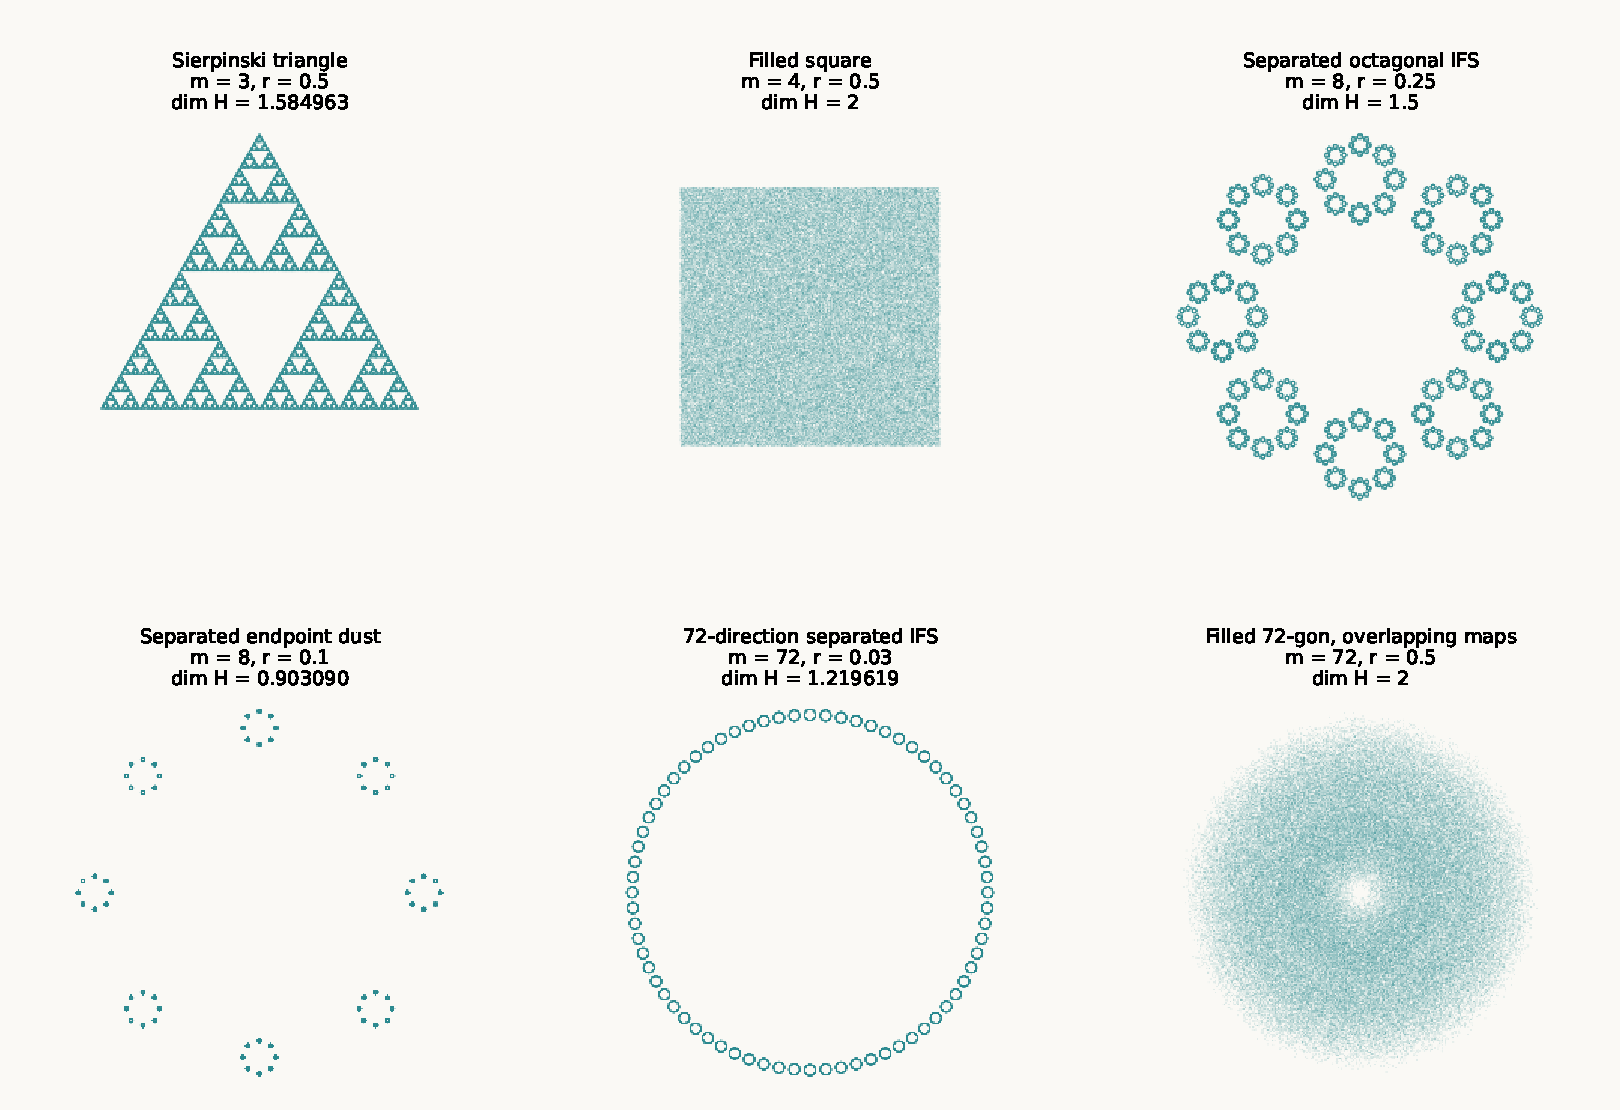
\includegraphics[width=\linewidth]{endpoint_variants.pdf}
\captionof{figure}{Each panel contains 120,000 chaos-game samples with
seed 20260930. These finite stochastic plots illustrate endpoint attractors,
not accumulated traces. A round-looking cluster is not a proof that a
circle or disk is filled. Dimensions below are justified analytically.}
\end{center}

\begin{center}
\small
\begin{tabular}{r r r r l}
\toprule
$m$ & $r$ & $\dimH K$ & $\dimH S$ & Certificate\\
\midrule
3 & 0.5 & 1.584963 & 1.584963 & Sierpinski triangle; OSC\\
4 & 0.5 & 2 & 2 & Four squares tile the square\\
8 & 0.25 & 1.5 & 1.5 & $r<q_8$\\
8 & 0.1 & 0.903090 & 1 & $r<q_8$\\
72 & 0.03 & 1.219619 & 1.219619 & $r<q_{72}$\\
72 & 0.5 & Undetermined & Undetermined & Overlaps; no claim here\\
\bottomrule
\end{tabular}
\end{center}

For the triangle at scale $1/2$, the three open corner triangles have
disjoint interiors inside the original triangle. The open set condition
therefore gives $\log 3/\log2$. For the square at scale $1/2$, the four
corner copies tile the entire square; uniqueness of the compact
attractor makes $K$ that square. A contractive IFS need not have a
noninteger dimension or a perforated attractor.

Values of $L$ translate coordinate units through a uniform scaling;
$\theta$ rotates the figure. Neither changes these dimensions. No
dimension is inferred from opacity, image resolution, repeated overdraw
or apparent empty regions in the point samples.

\newpage
% Page 8
\sectiontitle{7. Reference software and verification}
The package \texttt{adler\_fractal/} implements the definitions with
Python floating-point coordinates. Geometry and SVG export use only the
standard library. PNG output and the report figures use Matplotlib;
the supplied environment pins Matplotlib 3.10.8 and NumPy 2.3.5.
Geometry and SVG need Python 3.10 or later; the pinned figure environment
needs Python 3.11 or later.

\subsection*{Three output meanings}
\begin{description}[leftmargin=18mm,labelwidth=16mm,labelsep=2mm,font=\normalfont\ttfamily]
\item[\texttt{trace}] Enumerates every segment command through depth $n$,
preserving traversal order and multiplicity.
\item[\texttt{endpoints}] Enumerates depth-$n$ endpoint addresses, with
multiplicity; this is not a deduplicated point set.
\item[\texttt{chaos}] Samples $x_{t+1}=rx_t+Lu_{J_t}$ with uniform independent
direction choices and a recorded seed. It requires $0<r<1$; $n$ is irrelevant.
The automatic burn-in bounds initial-position error relative to the limiting
radius by $10^{-12}$. Sampling is not an exact attractor representation.
\end{description}

\subsection*{Checks performed}
All 12 tests in \texttt{tests/test\_geometry.py} pass. The principal
equivalence test executes the unchanged original drawing function with
an independent minimal Turtle recorder, avoiding a GUI. It compares all
5,256 segments in order with the reference output; start and end
coordinates agree within $10^{-10}$ length units. Further tests check
the explicit word formula, counts, generation lengths, sharp radii,
dihedral endpoint symmetry, second-generation multiplicities,
translation, adapter behavior, empty depth, invalid parameters,
SVG validity, budget rejection, seeded reproducibility and discipline
around uncertified dimension claims. Numerical tests support the
implementation; the infinite-set claims depend on the proofs.

\subsection*{Reproduction}
Run in the unpacked project directory:
\begin{verbatim}
python3 -m adler_fractal --output adler_original.svg
python3 -m adler_fractal --spokes 8 --scale 0.25 \
    --mode chaos --samples 100000 --output sample.svg
python3 -m unittest discover -s tests -v
python3 -m pip install -r requirements.txt
python3 scripts/make_figures.py
\end{verbatim}
The \LaTeX\ source can be built from \texttt{docs/} using two passes of
\texttt{xelatex}. The unchanged original and package checksums support
provenance and comparison. Test details are recorded in the included
\texttt{scripts/verification\_report.json}.

\subsection*{Resource and numerical limitations}
Enumeration takes time proportional to the number of commands or
addresses. The explicit traversal stack uses $O(mn)$ pending storage;
Matplotlib additionally collects rendered data in memory. SVG is streamed.
The default budget of one million rejects the depth-four original before
writing an SVG; it can be raised explicitly. Float rounding and rendering
choices do not change the exact mathematical definition.

\newpage
% Page 9
\sectiontitle{8. Related work, scope and publication status}
The contractive endpoint system is an established polygon-vertex IFS.
The trace closure is an established inhomogeneous self-similar set.
Hutchinson supplies the general compact-attractor and dimension theory
\cite{hutchinson}; Tzanov treats polygon and star-based IFS constructions
\cite{tzanov}; Fraser states the condensation-set decomposition and
Hausdorff-dimension rule \cite{fraser}. The equal-length density proof and
finite combinatorial calculations here provide direct analyses of the
supplied parameters, without asserting that these observations are first
discoveries.

The scoped literature check on 30 September 2026 included searches for
the proposed name, radial recursive stars, equal-length spoke drawings,
regular polygon IFS and inhomogeneous self-similar sets. The three listed
primary full texts were examined. This was not an exhaustive review of
MathSciNet, zbMATH, all books, code archives or unpublished work. An exact
earlier instance of the supplied finite Turtle program was not established
by this check. Absence of a located exact instance is not evidence of
historical priority.

\subsection*{Meaning of the proposed name}
\emph{Adler Fractal} is used here as a proposed descriptive name for the
documented construction and implementation. Finite drawings have dimension
one; the original's infinite closure is the plane; contractive limits
include dust, the classical Sierpinski triangle and a filled square.
The name does not imply that every parameter choice defines a new or
noninteger-dimensional fractal. Finiteness of a rendered picture alone
does not distinguish a fractal approximation from another finite drawing;
the underlying limiting rule and the specified set are what is analyzed here.

\subsection*{Deposition and licenses}
This version was prepared for public deposition on Zenodo with the German
specification, literature-check log, reference code and reproducible figures.
DOI \texttt{10.5281/zenodo.23057945} was actually reserved before file
preparation; Zenodo registers it upon publication \cite{zenodo}. Marcus Adler
authorized public deposition and selected MIT for software and CC BY 4.0
for original text and figures; the package specifies the respective scopes.
Independent peer review has not been performed. A DOI makes a deposited
record citable; it is not a novelty certificate, a peer review or an official
assignment of the name.

\begingroup
\small
\renewcommand{\refname}{\sffamily\color{ink}References}
\begin{thebibliography}{9}
\bibitem{hutchinson} J. E. Hutchinson.
\emph{Fractals and Self-Similarity}.
Indiana University Mathematics Journal 30 (1981), 713--747.
\href{https://doi.org/10.1512/iumj.1981.30.30055}{doi:10.1512/iumj.1981.30.30055}.

\bibitem{tzanov} V. Tzanov.
\emph{Strictly self-similar fractals composed of star-polygons that are
attractors of Iterated Function Systems} (2015).
\href{https://arxiv.org/abs/1502.01384}{arXiv:1502.01384}.

\bibitem{fraser} J. M. Fraser.
\emph{Inhomogeneous self-similar sets and box dimensions}.
Studia Mathematica 213 (2012), 133--156.
\href{https://arxiv.org/abs/1301.1881}{arXiv:1301.1881} (submitted 2013),
especially \S1.1.

\bibitem{zenodo} Zenodo.
\emph{Create new upload}. Official deposit documentation.
\url{https://help.zenodo.org/docs/deposit/create-new-upload/}.
Accessed 30 September 2026.
\end{thebibliography}
\endgroup

\end{document}
